% =====================================================================
% figA  — R/ggplot2 -> tikzDevice (parallel to ../figures-tex/figA_lawtransfer.tex)
% Canonical-JSON-only. Regenerate: Rscript figures-r/make_figures.R
% Provenance (JSON path :: field = plotted value), one line per series:
% SOURCE: results/G1_L8_analysis.json :: aggregate.within_probe_mean_across_seeds = 0.3951
% SOURCE: results/G1_L8_analysis.json :: mean(per_seed[].within_probe_mean_normgrowth) = 0.0825
% SOURCE: results/G1_L10_analysis.json :: aggregate.within_probe_mean_across_seeds = 0.5337
% SOURCE: results/G1_L10_analysis.json :: mean(per_seed[].within_probe_mean_normgrowth) = 0.2458
% SOURCE: results/G1_L12_analysis.json :: aggregate.within_probe_mean_across_seeds = 0.6018
% SOURCE: results/G1_L12_analysis.json :: mean(per_seed[].within_probe_mean_normgrowth) = 0.5087
% SOURCE: results/G1_L14_analysis.json :: aggregate.within_probe_mean_across_seeds = 0.3006
% SOURCE: results/G1_L14_analysis.json :: mean(per_seed[].within_probe_mean_normgrowth) = 0.5019
% SOURCE: results/C3_regime_3b_L24_r4.json :: aggregate.within_probe_mean_across_seeds = 0.3764
% SOURCE: results/C3_llama8b_r3.json :: per_seed[L16].within_probe_mean = 0.1734
% SOURCE: results/C3_llama8b_r3.json :: per_seed[L24].within_probe_mean = -0.1169
% SOURCE: results/C3_llama8b_r3.json :: per_seed[L28].within_probe_mean = 0.1554
% SOURCE: results/G1_L12_analysis.json :: aggregate.within_probe_mean_across_seeds = 0.6018
% SOURCE: results/C3_null_llama3b_L14.json :: aggregate.within_probe_mean_across_seeds = 0.2910
% SOURCE: results/C3_null_gemma2b_L13_v2.json :: aggregate.within_probe_mean_across_seeds = 0.0841
% SOURCE: results/C3_null_phi35_L16_v2.json :: aggregate.within_probe_mean_across_seeds = 0.0169
% SOURCE: results/C3_null_qwen05b_L12.json :: aggregate.within_probe_mean_across_seeds = 0.1030
% SOURCE: results/C3_null_qwen15b_L14.json :: aggregate.within_probe_mean_across_seeds = -0.1716
% SOURCE: results/C3_null_qwen3b_L18_v2.json :: aggregate.within_probe_mean_across_seeds = -0.1191
% SOURCE: results/C1_magnitude_table.json :: families[family=llama1b_L12].within_probe_mean_abs_across_seeds = 0.6133
% SOURCE: results/C1_magnitude_table.json :: families[family=gemma2b_L13].within_probe_mean_abs_across_seeds = 0.0858
% SOURCE: results/C1_magnitude_table.json :: families[family=phi35_L16].within_probe_mean_abs_across_seeds = 0.3214
% SOURCE: results/C1_magnitude_table.json :: families[family=qwen05b_L12].within_probe_mean_abs_across_seeds = 0.3197
% SOURCE: results/C1_magnitude_table.json :: families[family=qwen15b_L14].within_probe_mean_abs_across_seeds = 0.4124
% SOURCE: results/C1_magnitude_table.json :: families[family=qwen3b_L18].within_probe_mean_abs_across_seeds = 0.4013
% =====================================================================
% !TEX encoding = UTF-8 Unicode
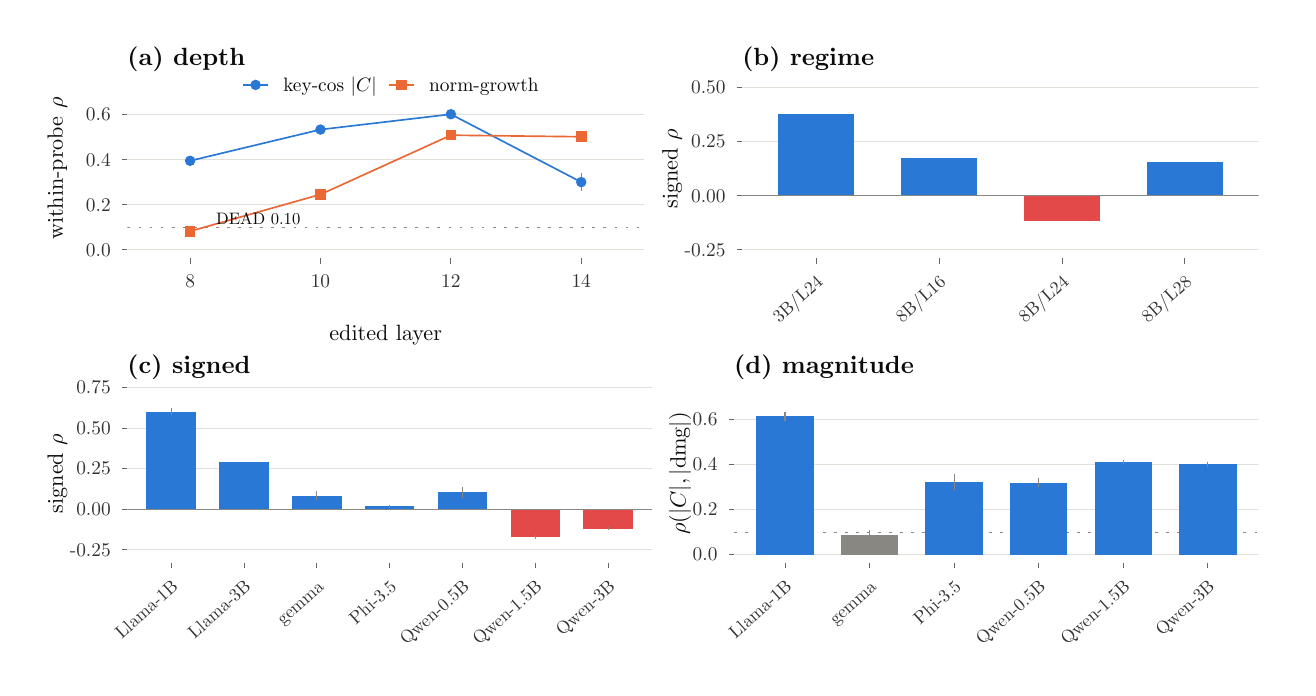
\begin{tikzpicture}[x=1pt,y=1pt]
\definecolor{fillColor}{RGB}{255,255,255}
\path[use as bounding box,fill=fillColor,fill opacity=0.00] (0,0) rectangle (455.30,231.26);
\begin{scope}
\path[clip] (  0.00,  0.00) rectangle (455.30,231.26);
\definecolor{drawColor}{RGB}{255,255,255}
\definecolor{fillColor}{RGB}{255,255,255}

\path[draw=drawColor,line width= 0.6pt,line join=round,line cap=round,fill=fillColor] (  0.00, -0.00) rectangle (455.30,231.26);
\end{scope}
\begin{scope}
\path[clip] (  5.50,114.57) rectangle (227.65,225.76);
\definecolor{fillColor}{RGB}{255,255,255}

\path[fill=fillColor] (  5.50,114.57) rectangle (227.65,225.76);
\end{scope}
\begin{scope}
\path[clip] (227.65,114.57) rectangle (449.80,225.76);
\definecolor{fillColor}{RGB}{255,255,255}

\path[fill=fillColor] (227.65,114.57) rectangle (449.80,225.76);
\end{scope}
\begin{scope}
\path[clip] ( 36.07,148.04) rectangle (222.65,212.54);
\definecolor{drawColor}{RGB}{225,224,217}

\path[draw=drawColor,line width= 0.3pt,line join=round] ( 36.07,150.97) --
	(222.65,150.97);

\path[draw=drawColor,line width= 0.3pt,line join=round] ( 36.07,167.26) --
	(222.65,167.26);

\path[draw=drawColor,line width= 0.3pt,line join=round] ( 36.07,183.55) --
	(222.65,183.55);

\path[draw=drawColor,line width= 0.3pt,line join=round] ( 36.07,199.84) --
	(222.65,199.84);
\definecolor{drawColor}{RGB}{137,135,129}

\path[draw=drawColor,line width= 0.3pt,dash pattern=on 1pt off 3pt ,line join=round] ( 36.07,159.11) -- (222.65,159.11);

\path[draw=drawColor,line width= 0.4pt,line join=round] ( 58.69,184.01) --
	( 58.69,184.01);

\path[draw=drawColor,line width= 0.4pt,line join=round] ( 58.69,184.01) --
	( 58.69,182.29);

\path[draw=drawColor,line width= 0.4pt,line join=round] ( 58.69,182.29) --
	( 58.69,182.29);

\path[draw=drawColor,line width= 0.4pt,line join=round] (105.80,195.29) --
	(105.80,195.29);

\path[draw=drawColor,line width= 0.4pt,line join=round] (105.80,195.29) --
	(105.80,193.58);

\path[draw=drawColor,line width= 0.4pt,line join=round] (105.80,193.58) --
	(105.80,193.58);

\path[draw=drawColor,line width= 0.4pt,line join=round] (152.92,201.52) --
	(152.92,201.52);

\path[draw=drawColor,line width= 0.4pt,line join=round] (152.92,201.52) --
	(152.92,198.44);

\path[draw=drawColor,line width= 0.4pt,line join=round] (152.92,198.44) --
	(152.92,198.44);

\path[draw=drawColor,line width= 0.4pt,line join=round] (200.03,178.73) --
	(200.03,178.73);

\path[draw=drawColor,line width= 0.4pt,line join=round] (200.03,178.73) --
	(200.03,172.17);

\path[draw=drawColor,line width= 0.4pt,line join=round] (200.03,172.17) --
	(200.03,172.17);
\definecolor{drawColor}{RGB}{42,120,214}

\path[draw=drawColor,line width= 0.6pt,line join=round] ( 58.69,183.15) --
	(105.80,194.44) --
	(152.92,199.98) --
	(200.03,175.45);
\definecolor{drawColor}{RGB}{235,104,52}

\path[draw=drawColor,line width= 0.6pt,line join=round] ( 58.69,157.69) --
	(105.80,170.99) --
	(152.92,192.40) --
	(200.03,191.84);
\definecolor{fillColor}{RGB}{42,120,214}

\path[fill=fillColor] ( 58.69,183.15) circle (  1.90);

\path[fill=fillColor] (105.80,194.44) circle (  1.90);

\path[fill=fillColor] (152.92,199.98) circle (  1.90);

\path[fill=fillColor] (200.03,175.45) circle (  1.90);
\definecolor{fillColor}{RGB}{235,104,52}

\path[fill=fillColor] ( 56.79,155.79) --
	( 60.58,155.79) --
	( 60.58,159.59) --
	( 56.79,159.59) --
	cycle;

\path[fill=fillColor] (103.91,169.09) --
	(107.70,169.09) --
	(107.70,172.89) --
	(103.91,172.89) --
	cycle;

\path[fill=fillColor] (151.02,190.51) --
	(154.82,190.51) --
	(154.82,194.30) --
	(151.02,194.30) --
	cycle;

\path[fill=fillColor] (198.14,189.95) --
	(201.93,189.95) --
	(201.93,193.74) --
	(198.14,193.74) --
	cycle;
\definecolor{drawColor}{RGB}{11,11,11}

\node[text=drawColor,anchor=base west,inner sep=0pt, outer sep=0pt, scale=  0.60] at ( 68.11,160.02) {DEAD 0.10};
\end{scope}
\begin{scope}
\path[clip] (  0.00,  0.00) rectangle (455.30,231.26);
\definecolor{drawColor}{gray}{0.20}

\node[text=drawColor,anchor=base east,inner sep=0pt, outer sep=0pt, scale=  0.70] at ( 30.02,148.69) {0.0};

\node[text=drawColor,anchor=base east,inner sep=0pt, outer sep=0pt, scale=  0.70] at ( 30.02,164.98) {0.2};

\node[text=drawColor,anchor=base east,inner sep=0pt, outer sep=0pt, scale=  0.70] at ( 30.02,181.27) {0.4};

\node[text=drawColor,anchor=base east,inner sep=0pt, outer sep=0pt, scale=  0.70] at ( 30.02,197.56) {0.6};
\end{scope}
\begin{scope}
\path[clip] (  0.00,  0.00) rectangle (455.30,231.26);
\definecolor{drawColor}{gray}{0.40}

\path[draw=drawColor,line width= 0.3pt,line join=round] ( 34.07,150.97) --
	( 36.07,150.97);

\path[draw=drawColor,line width= 0.3pt,line join=round] ( 34.07,167.26) --
	( 36.07,167.26);

\path[draw=drawColor,line width= 0.3pt,line join=round] ( 34.07,183.55) --
	( 36.07,183.55);

\path[draw=drawColor,line width= 0.3pt,line join=round] ( 34.07,199.84) --
	( 36.07,199.84);
\end{scope}
\begin{scope}
\path[clip] (  0.00,  0.00) rectangle (455.30,231.26);
\definecolor{drawColor}{gray}{0.40}

\path[draw=drawColor,line width= 0.3pt,line join=round] ( 58.69,146.04) --
	( 58.69,148.04);

\path[draw=drawColor,line width= 0.3pt,line join=round] (105.80,146.04) --
	(105.80,148.04);

\path[draw=drawColor,line width= 0.3pt,line join=round] (152.92,146.04) --
	(152.92,148.04);

\path[draw=drawColor,line width= 0.3pt,line join=round] (200.03,146.04) --
	(200.03,148.04);
\end{scope}
\begin{scope}
\path[clip] (  0.00,  0.00) rectangle (455.30,231.26);
\definecolor{drawColor}{gray}{0.20}

\node[text=drawColor,anchor=base,inner sep=0pt, outer sep=0pt, scale=  0.70] at ( 58.69,137.43) {8};

\node[text=drawColor,anchor=base,inner sep=0pt, outer sep=0pt, scale=  0.70] at (105.80,137.43) {10};

\node[text=drawColor,anchor=base,inner sep=0pt, outer sep=0pt, scale=  0.70] at (152.92,137.43) {12};

\node[text=drawColor,anchor=base,inner sep=0pt, outer sep=0pt, scale=  0.70] at (200.03,137.43) {14};
\end{scope}
\begin{scope}
\path[clip] (  0.00,  0.00) rectangle (455.30,231.26);
\definecolor{drawColor}{RGB}{11,11,11}

\node[text=drawColor,anchor=base,inner sep=0pt, outer sep=0pt, scale=  0.80] at (129.36,118.30) {edited layer};
\end{scope}
\begin{scope}
\path[clip] (  0.00,  0.00) rectangle (455.30,231.26);
\definecolor{drawColor}{RGB}{11,11,11}

\node[text=drawColor,rotate= 90.00,anchor=base,inner sep=0pt, outer sep=0pt, scale=  0.80] at ( 12.71,180.29) {within-probe $\rho$};
\end{scope}
\begin{scope}
\path[clip] (  0.00,  0.00) rectangle (455.30,231.26);
\definecolor{drawColor}{RGB}{42,120,214}

\path[draw=drawColor,line width= 0.6pt,line join=round] ( 77.96,210.58) -- ( 86.76,210.58);
\definecolor{fillColor}{RGB}{42,120,214}

\path[fill=fillColor] ( 82.36,210.58) circle (  1.90);
\end{scope}
\begin{scope}
\path[clip] (  0.00,  0.00) rectangle (455.30,231.26);
\definecolor{drawColor}{RGB}{235,104,52}

\path[draw=drawColor,line width= 0.6pt,line join=round] (130.70,210.58) -- (139.50,210.58);
\definecolor{fillColor}{RGB}{235,104,52}

\path[fill=fillColor] (133.20,208.68) --
	(136.99,208.68) --
	(136.99,212.48) --
	(133.20,212.48) --
	cycle;
\end{scope}
\begin{scope}
\path[clip] (  0.00,  0.00) rectangle (455.30,231.26);
\definecolor{drawColor}{RGB}{11,11,11}

\node[text=drawColor,anchor=base west,inner sep=0pt, outer sep=0pt, scale=  0.70] at ( 92.36,208.30) {key-cos $|C|$};
\end{scope}
\begin{scope}
\path[clip] (  0.00,  0.00) rectangle (455.30,231.26);
\definecolor{drawColor}{RGB}{11,11,11}

\node[text=drawColor,anchor=base west,inner sep=0pt, outer sep=0pt, scale=  0.70] at (145.10,208.30) {norm-growth};
\end{scope}
\begin{scope}
\path[clip] (  0.00,  0.00) rectangle (455.30,231.26);
\definecolor{drawColor}{RGB}{11,11,11}

\node[text=drawColor,anchor=base west,inner sep=0pt, outer sep=0pt, scale=  0.90] at ( 36.07,217.56) {\bfseries (a) depth};
\end{scope}
\begin{scope}
\path[clip] (258.22,148.04) rectangle (444.80,212.54);
\definecolor{drawColor}{RGB}{225,224,217}

\path[draw=drawColor,line width= 0.3pt,line join=round] (258.22,150.97) --
	(444.80,150.97);

\path[draw=drawColor,line width= 0.3pt,line join=round] (258.22,170.52) --
	(444.80,170.52);

\path[draw=drawColor,line width= 0.3pt,line join=round] (258.22,190.06) --
	(444.80,190.06);

\path[draw=drawColor,line width= 0.3pt,line join=round] (258.22,209.61) --
	(444.80,209.61);
\definecolor{fillColor}{RGB}{42,120,214}

\path[fill=fillColor] (271.10,170.52) rectangle (298.65,199.95);

\path[fill=fillColor] (315.53,170.52) rectangle (343.07,184.07);
\definecolor{fillColor}{RGB}{227,73,72}

\path[fill=fillColor] (359.95,161.38) rectangle (387.49,170.52);
\definecolor{fillColor}{RGB}{42,120,214}

\path[fill=fillColor] (404.38,170.52) rectangle (431.92,182.67);
\definecolor{drawColor}{RGB}{137,135,129}

\path[draw=drawColor,line width= 0.3pt,line join=round] (258.22,170.52) -- (444.80,170.52);
\end{scope}
\begin{scope}
\path[clip] (  0.00,  0.00) rectangle (455.30,231.26);
\definecolor{drawColor}{gray}{0.20}

\node[text=drawColor,anchor=base east,inner sep=0pt, outer sep=0pt, scale=  0.70] at (252.17,148.69) {-0.25};

\node[text=drawColor,anchor=base east,inner sep=0pt, outer sep=0pt, scale=  0.70] at (252.17,168.24) {0.00};

\node[text=drawColor,anchor=base east,inner sep=0pt, outer sep=0pt, scale=  0.70] at (252.17,187.79) {0.25};

\node[text=drawColor,anchor=base east,inner sep=0pt, outer sep=0pt, scale=  0.70] at (252.17,207.33) {0.50};
\end{scope}
\begin{scope}
\path[clip] (  0.00,  0.00) rectangle (455.30,231.26);
\definecolor{drawColor}{gray}{0.40}

\path[draw=drawColor,line width= 0.3pt,line join=round] (256.22,150.97) --
	(258.22,150.97);

\path[draw=drawColor,line width= 0.3pt,line join=round] (256.22,170.52) --
	(258.22,170.52);

\path[draw=drawColor,line width= 0.3pt,line join=round] (256.22,190.06) --
	(258.22,190.06);

\path[draw=drawColor,line width= 0.3pt,line join=round] (256.22,209.61) --
	(258.22,209.61);
\end{scope}
\begin{scope}
\path[clip] (  0.00,  0.00) rectangle (455.30,231.26);
\definecolor{drawColor}{gray}{0.40}

\path[draw=drawColor,line width= 0.3pt,line join=round] (284.88,146.04) --
	(284.88,148.04);

\path[draw=drawColor,line width= 0.3pt,line join=round] (329.30,146.04) --
	(329.30,148.04);

\path[draw=drawColor,line width= 0.3pt,line join=round] (373.72,146.04) --
	(373.72,148.04);

\path[draw=drawColor,line width= 0.3pt,line join=round] (418.15,146.04) --
	(418.15,148.04);
\end{scope}
\begin{scope}
\path[clip] (  0.00,  0.00) rectangle (455.30,231.26);
\definecolor{drawColor}{gray}{0.20}

\node[text=drawColor,rotate= 42.00,anchor=base east,inner sep=0pt, outer sep=0pt, scale=  0.65] at (287.71,138.84) {3B/L24};

\node[text=drawColor,rotate= 42.00,anchor=base east,inner sep=0pt, outer sep=0pt, scale=  0.65] at (332.13,138.84) {8B/L16};

\node[text=drawColor,rotate= 42.00,anchor=base east,inner sep=0pt, outer sep=0pt, scale=  0.65] at (376.55,138.84) {8B/L24};

\node[text=drawColor,rotate= 42.00,anchor=base east,inner sep=0pt, outer sep=0pt, scale=  0.65] at (420.98,138.84) {8B/L28};
\end{scope}
\begin{scope}
\path[clip] (  0.00,  0.00) rectangle (455.30,231.26);
\definecolor{drawColor}{RGB}{11,11,11}

\node[text=drawColor,rotate= 90.00,anchor=base,inner sep=0pt, outer sep=0pt, scale=  0.80] at (234.86,180.29) {signed $\rho$};
\end{scope}
\begin{scope}
\path[clip] (  0.00,  0.00) rectangle (455.30,231.26);
\definecolor{drawColor}{RGB}{11,11,11}

\node[text=drawColor,anchor=base west,inner sep=0pt, outer sep=0pt, scale=  0.90] at (258.22,217.56) {\bfseries (b) regime};
\end{scope}
\begin{scope}
\path[clip] (  5.50,  5.50) rectangle (230.57,114.57);
\definecolor{fillColor}{RGB}{255,255,255}

\path[fill=fillColor] (  5.50,  5.50) rectangle (230.57,114.57);
\end{scope}
\begin{scope}
\path[clip] (230.57,  5.50) rectangle (449.80,114.57);
\definecolor{fillColor}{RGB}{255,255,255}

\path[fill=fillColor] (230.57,  5.50) rectangle (449.80,114.57);
\end{scope}
\begin{scope}
\path[clip] ( 36.07, 37.91) rectangle (225.57,102.42);
\definecolor{drawColor}{RGB}{225,224,217}

\path[draw=drawColor,line width= 0.3pt,line join=round] ( 36.07, 42.60) --
	(225.57, 42.60);

\path[draw=drawColor,line width= 0.3pt,line join=round] ( 36.07, 57.26) --
	(225.57, 57.26);

\path[draw=drawColor,line width= 0.3pt,line join=round] ( 36.07, 71.92) --
	(225.57, 71.92);

\path[draw=drawColor,line width= 0.3pt,line join=round] ( 36.07, 86.58) --
	(225.57, 86.58);

\path[draw=drawColor,line width= 0.3pt,line join=round] ( 36.07,101.24) --
	(225.57,101.24);
\definecolor{fillColor}{RGB}{42,120,214}

\path[fill=fillColor] ( 42.91, 57.26) rectangle ( 60.81, 92.55);

\path[fill=fillColor] ( 69.23, 57.26) rectangle ( 87.13, 74.33);

\path[fill=fillColor] ( 95.55, 57.26) rectangle (113.45, 62.20);

\path[fill=fillColor] (121.87, 57.26) rectangle (139.77, 58.25);

\path[fill=fillColor] (148.19, 57.26) rectangle (166.09, 63.30);
\definecolor{fillColor}{RGB}{227,73,72}

\path[fill=fillColor] (174.51, 47.20) rectangle (192.40, 57.26);

\path[fill=fillColor] (200.83, 50.28) rectangle (218.72, 57.26);
\definecolor{drawColor}{RGB}{137,135,129}

\path[draw=drawColor,line width= 0.3pt,line join=round] ( 36.07, 57.26) -- (225.57, 57.26);

\path[draw=drawColor,line width= 0.4pt,line join=round] ( 51.86, 93.66) --
	( 51.86, 93.66);

\path[draw=drawColor,line width= 0.4pt,line join=round] ( 51.86, 93.66) --
	( 51.86, 91.45);

\path[draw=drawColor,line width= 0.4pt,line join=round] ( 51.86, 91.45) --
	( 51.86, 91.45);

\path[draw=drawColor,line width= 0.4pt,line join=round] (104.50, 63.92) --
	(104.50, 63.92);

\path[draw=drawColor,line width= 0.4pt,line join=round] (104.50, 63.92) --
	(104.50, 60.47);

\path[draw=drawColor,line width= 0.4pt,line join=round] (104.50, 60.47) --
	(104.50, 60.47);

\path[draw=drawColor,line width= 0.4pt,line join=round] (130.82, 58.77) --
	(130.82, 58.77);

\path[draw=drawColor,line width= 0.4pt,line join=round] (130.82, 58.77) --
	(130.82, 57.74);

\path[draw=drawColor,line width= 0.4pt,line join=round] (130.82, 57.74) --
	(130.82, 57.74);

\path[draw=drawColor,line width= 0.4pt,line join=round] (157.14, 65.23) --
	(157.14, 65.23);

\path[draw=drawColor,line width= 0.4pt,line join=round] (157.14, 65.23) --
	(157.14, 61.37);

\path[draw=drawColor,line width= 0.4pt,line join=round] (157.14, 61.37) --
	(157.14, 61.37);

\path[draw=drawColor,line width= 0.4pt,line join=round] (183.46, 47.93) --
	(183.46, 47.93);

\path[draw=drawColor,line width= 0.4pt,line join=round] (183.46, 47.93) --
	(183.46, 46.47);

\path[draw=drawColor,line width= 0.4pt,line join=round] (183.46, 46.47) --
	(183.46, 46.47);

\path[draw=drawColor,line width= 0.4pt,line join=round] (209.77, 50.68) --
	(209.77, 50.68);

\path[draw=drawColor,line width= 0.4pt,line join=round] (209.77, 50.68) --
	(209.77, 49.88);

\path[draw=drawColor,line width= 0.4pt,line join=round] (209.77, 49.88) --
	(209.77, 49.88);
\end{scope}
\begin{scope}
\path[clip] (  0.00,  0.00) rectangle (455.30,231.26);
\definecolor{drawColor}{gray}{0.20}

\node[text=drawColor,anchor=base east,inner sep=0pt, outer sep=0pt, scale=  0.70] at ( 30.02, 40.33) {-0.25};

\node[text=drawColor,anchor=base east,inner sep=0pt, outer sep=0pt, scale=  0.70] at ( 30.02, 54.99) {0.00};

\node[text=drawColor,anchor=base east,inner sep=0pt, outer sep=0pt, scale=  0.70] at ( 30.02, 69.65) {0.25};

\node[text=drawColor,anchor=base east,inner sep=0pt, outer sep=0pt, scale=  0.70] at ( 30.02, 84.31) {0.50};

\node[text=drawColor,anchor=base east,inner sep=0pt, outer sep=0pt, scale=  0.70] at ( 30.02, 98.97) {0.75};
\end{scope}
\begin{scope}
\path[clip] (  0.00,  0.00) rectangle (455.30,231.26);
\definecolor{drawColor}{gray}{0.40}

\path[draw=drawColor,line width= 0.3pt,line join=round] ( 34.07, 42.60) --
	( 36.07, 42.60);

\path[draw=drawColor,line width= 0.3pt,line join=round] ( 34.07, 57.26) --
	( 36.07, 57.26);

\path[draw=drawColor,line width= 0.3pt,line join=round] ( 34.07, 71.92) --
	( 36.07, 71.92);

\path[draw=drawColor,line width= 0.3pt,line join=round] ( 34.07, 86.58) --
	( 36.07, 86.58);

\path[draw=drawColor,line width= 0.3pt,line join=round] ( 34.07,101.24) --
	( 36.07,101.24);
\end{scope}
\begin{scope}
\path[clip] (  0.00,  0.00) rectangle (455.30,231.26);
\definecolor{drawColor}{gray}{0.40}

\path[draw=drawColor,line width= 0.3pt,line join=round] ( 51.86, 35.91) --
	( 51.86, 37.91);

\path[draw=drawColor,line width= 0.3pt,line join=round] ( 78.18, 35.91) --
	( 78.18, 37.91);

\path[draw=drawColor,line width= 0.3pt,line join=round] (104.50, 35.91) --
	(104.50, 37.91);

\path[draw=drawColor,line width= 0.3pt,line join=round] (130.82, 35.91) --
	(130.82, 37.91);

\path[draw=drawColor,line width= 0.3pt,line join=round] (157.14, 35.91) --
	(157.14, 37.91);

\path[draw=drawColor,line width= 0.3pt,line join=round] (183.46, 35.91) --
	(183.46, 37.91);

\path[draw=drawColor,line width= 0.3pt,line join=round] (209.77, 35.91) --
	(209.77, 37.91);
\end{scope}
\begin{scope}
\path[clip] (  0.00,  0.00) rectangle (455.30,231.26);
\definecolor{drawColor}{gray}{0.20}

\node[text=drawColor,rotate= 42.00,anchor=base east,inner sep=0pt, outer sep=0pt, scale=  0.65] at ( 54.69, 28.72) {Llama-1B};

\node[text=drawColor,rotate= 42.00,anchor=base east,inner sep=0pt, outer sep=0pt, scale=  0.65] at ( 81.01, 28.72) {Llama-3B};

\node[text=drawColor,rotate= 42.00,anchor=base east,inner sep=0pt, outer sep=0pt, scale=  0.65] at (107.33, 28.72) {gemma};

\node[text=drawColor,rotate= 42.00,anchor=base east,inner sep=0pt, outer sep=0pt, scale=  0.65] at (133.65, 28.72) {Phi-3.5};

\node[text=drawColor,rotate= 42.00,anchor=base east,inner sep=0pt, outer sep=0pt, scale=  0.65] at (159.97, 28.72) {Qwen-0.5B};

\node[text=drawColor,rotate= 42.00,anchor=base east,inner sep=0pt, outer sep=0pt, scale=  0.65] at (186.29, 28.72) {Qwen-1.5B};

\node[text=drawColor,rotate= 42.00,anchor=base east,inner sep=0pt, outer sep=0pt, scale=  0.65] at (212.61, 28.72) {Qwen-3B};
\end{scope}
\begin{scope}
\path[clip] (  0.00,  0.00) rectangle (455.30,231.26);
\definecolor{drawColor}{RGB}{11,11,11}

\node[text=drawColor,rotate= 90.00,anchor=base,inner sep=0pt, outer sep=0pt, scale=  0.80] at ( 12.71, 70.16) {signed $\rho$};
\end{scope}
\begin{scope}
\path[clip] (  0.00,  0.00) rectangle (455.30,231.26);
\definecolor{drawColor}{RGB}{11,11,11}

\node[text=drawColor,anchor=base west,inner sep=0pt, outer sep=0pt, scale=  0.90] at ( 36.07,106.37) {\bfseries (c) signed};
\end{scope}
\begin{scope}
\path[clip] (255.31, 37.91) rectangle (444.80,102.42);
\definecolor{drawColor}{RGB}{225,224,217}

\path[draw=drawColor,line width= 0.3pt,line join=round] (255.31, 40.84) --
	(444.80, 40.84);

\path[draw=drawColor,line width= 0.3pt,line join=round] (255.31, 57.13) --
	(444.80, 57.13);

\path[draw=drawColor,line width= 0.3pt,line join=round] (255.31, 73.42) --
	(444.80, 73.42);

\path[draw=drawColor,line width= 0.3pt,line join=round] (255.31, 89.71) --
	(444.80, 89.71);
\definecolor{drawColor}{RGB}{137,135,129}

\path[draw=drawColor,line width= 0.3pt,dash pattern=on 1pt off 3pt ,line join=round] (255.31, 48.99) -- (444.80, 48.99);
\definecolor{fillColor}{RGB}{42,120,214}

\path[fill=fillColor] (263.25, 40.84) rectangle (284.04, 90.79);
\definecolor{fillColor}{RGB}{137,135,129}

\path[fill=fillColor] (293.82, 40.84) rectangle (314.60, 47.83);
\definecolor{fillColor}{RGB}{42,120,214}

\path[fill=fillColor] (324.38, 40.84) rectangle (345.16, 67.02);

\path[fill=fillColor] (354.94, 40.84) rectangle (375.73, 66.88);

\path[fill=fillColor] (385.51, 40.84) rectangle (406.29, 74.43);

\path[fill=fillColor] (416.07, 40.84) rectangle (436.85, 73.53);

\path[draw=drawColor,line width= 0.4pt,line join=round] (273.64, 92.31) --
	(273.64, 92.31);

\path[draw=drawColor,line width= 0.4pt,line join=round] (273.64, 92.31) --
	(273.64, 89.28);

\path[draw=drawColor,line width= 0.4pt,line join=round] (273.64, 89.28) --
	(273.64, 89.28);

\path[draw=drawColor,line width= 0.4pt,line join=round] (304.21, 49.87) --
	(304.21, 49.87);

\path[draw=drawColor,line width= 0.4pt,line join=round] (304.21, 49.87) --
	(304.21, 45.80);

\path[draw=drawColor,line width= 0.4pt,line join=round] (304.21, 45.80) --
	(304.21, 45.80);

\path[draw=drawColor,line width= 0.4pt,line join=round] (334.77, 69.88) --
	(334.77, 69.88);

\path[draw=drawColor,line width= 0.4pt,line join=round] (334.77, 69.88) --
	(334.77, 64.16);

\path[draw=drawColor,line width= 0.4pt,line join=round] (334.77, 64.16) --
	(334.77, 64.16);

\path[draw=drawColor,line width= 0.4pt,line join=round] (365.34, 68.61) --
	(365.34, 68.61);

\path[draw=drawColor,line width= 0.4pt,line join=round] (365.34, 68.61) --
	(365.34, 65.16);

\path[draw=drawColor,line width= 0.4pt,line join=round] (365.34, 65.16) --
	(365.34, 65.16);

\path[draw=drawColor,line width= 0.4pt,line join=round] (395.90, 75.13) --
	(395.90, 75.13);

\path[draw=drawColor,line width= 0.4pt,line join=round] (395.90, 75.13) --
	(395.90, 73.73);

\path[draw=drawColor,line width= 0.4pt,line join=round] (395.90, 73.73) --
	(395.90, 73.73);

\path[draw=drawColor,line width= 0.4pt,line join=round] (426.46, 74.42) --
	(426.46, 74.42);

\path[draw=drawColor,line width= 0.4pt,line join=round] (426.46, 74.42) --
	(426.46, 72.63);

\path[draw=drawColor,line width= 0.4pt,line join=round] (426.46, 72.63) --
	(426.46, 72.63);
\end{scope}
\begin{scope}
\path[clip] (  0.00,  0.00) rectangle (455.30,231.26);
\definecolor{drawColor}{gray}{0.20}

\node[text=drawColor,anchor=base east,inner sep=0pt, outer sep=0pt, scale=  0.70] at (249.26, 38.57) {0.0};

\node[text=drawColor,anchor=base east,inner sep=0pt, outer sep=0pt, scale=  0.70] at (249.26, 54.85) {0.2};

\node[text=drawColor,anchor=base east,inner sep=0pt, outer sep=0pt, scale=  0.70] at (249.26, 71.14) {0.4};

\node[text=drawColor,anchor=base east,inner sep=0pt, outer sep=0pt, scale=  0.70] at (249.26, 87.43) {0.6};
\end{scope}
\begin{scope}
\path[clip] (  0.00,  0.00) rectangle (455.30,231.26);
\definecolor{drawColor}{gray}{0.40}

\path[draw=drawColor,line width= 0.3pt,line join=round] (253.31, 40.84) --
	(255.31, 40.84);

\path[draw=drawColor,line width= 0.3pt,line join=round] (253.31, 57.13) --
	(255.31, 57.13);

\path[draw=drawColor,line width= 0.3pt,line join=round] (253.31, 73.42) --
	(255.31, 73.42);

\path[draw=drawColor,line width= 0.3pt,line join=round] (253.31, 89.71) --
	(255.31, 89.71);
\end{scope}
\begin{scope}
\path[clip] (  0.00,  0.00) rectangle (455.30,231.26);
\definecolor{drawColor}{gray}{0.40}

\path[draw=drawColor,line width= 0.3pt,line join=round] (273.64, 35.91) --
	(273.64, 37.91);

\path[draw=drawColor,line width= 0.3pt,line join=round] (304.21, 35.91) --
	(304.21, 37.91);

\path[draw=drawColor,line width= 0.3pt,line join=round] (334.77, 35.91) --
	(334.77, 37.91);

\path[draw=drawColor,line width= 0.3pt,line join=round] (365.34, 35.91) --
	(365.34, 37.91);

\path[draw=drawColor,line width= 0.3pt,line join=round] (395.90, 35.91) --
	(395.90, 37.91);

\path[draw=drawColor,line width= 0.3pt,line join=round] (426.46, 35.91) --
	(426.46, 37.91);
\end{scope}
\begin{scope}
\path[clip] (  0.00,  0.00) rectangle (455.30,231.26);
\definecolor{drawColor}{gray}{0.20}

\node[text=drawColor,rotate= 42.00,anchor=base east,inner sep=0pt, outer sep=0pt, scale=  0.65] at (276.48, 28.72) {Llama-1B};

\node[text=drawColor,rotate= 42.00,anchor=base east,inner sep=0pt, outer sep=0pt, scale=  0.65] at (307.04, 28.72) {gemma};

\node[text=drawColor,rotate= 42.00,anchor=base east,inner sep=0pt, outer sep=0pt, scale=  0.65] at (337.60, 28.72) {Phi-3.5};

\node[text=drawColor,rotate= 42.00,anchor=base east,inner sep=0pt, outer sep=0pt, scale=  0.65] at (368.17, 28.72) {Qwen-0.5B};

\node[text=drawColor,rotate= 42.00,anchor=base east,inner sep=0pt, outer sep=0pt, scale=  0.65] at (398.73, 28.72) {Qwen-1.5B};

\node[text=drawColor,rotate= 42.00,anchor=base east,inner sep=0pt, outer sep=0pt, scale=  0.65] at (429.29, 28.72) {Qwen-3B};
\end{scope}
\begin{scope}
\path[clip] (  0.00,  0.00) rectangle (455.30,231.26);
\definecolor{drawColor}{RGB}{11,11,11}

\node[text=drawColor,rotate= 90.00,anchor=base,inner sep=0pt, outer sep=0pt, scale=  0.80] at (237.77, 70.16) {$\rho(|C|,|$dmg$|)$};
\end{scope}
\begin{scope}
\path[clip] (  0.00,  0.00) rectangle (455.30,231.26);
\definecolor{drawColor}{RGB}{11,11,11}

\node[text=drawColor,anchor=base west,inner sep=0pt, outer sep=0pt, scale=  0.90] at (255.31,106.37) {\bfseries (d) magnitude};
\end{scope}
\end{tikzpicture}
